%%%%%%%%%%%%%%%%%%%%%%%%%%%%%%%%%%%%%%%%%%%%%%%%%%%%%%%%%%%%%%%%%%%%%%%%%%%%%%%%

%%%%%%%%%%%%%%%%%%%%%%%%%%%%%%%%%%%%%%%%%%%%%%%%%%%%%%%%%%%%%%%%%%%%%%%%%%%%%%%%
From the start of this dissertation we discussed how yield mapping is emerging as an important task in agricultural automation~\cite{hung2015feature,wang,das2015devices,deepApple,roy2016counting,roy2016surveying,peng2016semantic}. We have dedicated Chapters~\ref{chapter:detection} - \ref{chapter:map_yield} to the development of practical solutions for yield mapping. Current systems for automated yield mapping including ours involve the capture of imagery along an arbitrary and/or predetermined path. This approach is sufficient for large commercial orchards that have ``fruit-walls" where the fruit is visible from the outside. However, in more general settings, estimating the exact count from an arbitrary view is difficult. See Fig.~\ref{fig:compl}.


In this chapter, we show how active vision techniques can be used to accurately obtain the number of fruit in a cluster. Consider a system where a robot equipped with a controllable camera is charged with surveying an orchard (Fig.~\ref{fig:robotplatform}). Imagine that the robot positions the base near a tree and obtains the first view of an apple cluster. Where should it take the second image from so as to accurately estimate the number of apples in the cluster? We study this novel active perception problem.

Our approach can be summarized as follows: Consider the set of all possible ``world states" where each world state encodes the position and diameter of each fruit. The images acquired by the robot associate likelihoods to these world views. The goal is to plan views that reduce the entropy of this distribution sufficiently so that we can estimate the count accurately.  Directly enumerating all such world states is computationally expensive: In a $1m \times 1m \times 1m$ volume, a 1cm resolution grid would have $10^6$ cells. Even if we assume that the diameter is fixed, for a cluster of 6 fruit, there would be $10^{36}$ hypotheses. Our main contributions are (1)~a technique to efficiently enumerate only combinatorially distinct world states, and (2)~a method to estimate their likelihoods from these images. We experimentally demonstrate that together these methods yield an efficient view planning method for counting spherical objects which can be used in agricultural applications.



 


\begin{figure}[htb]
\centering
\begin{subfigure}[t]{0.3\textwidth}
    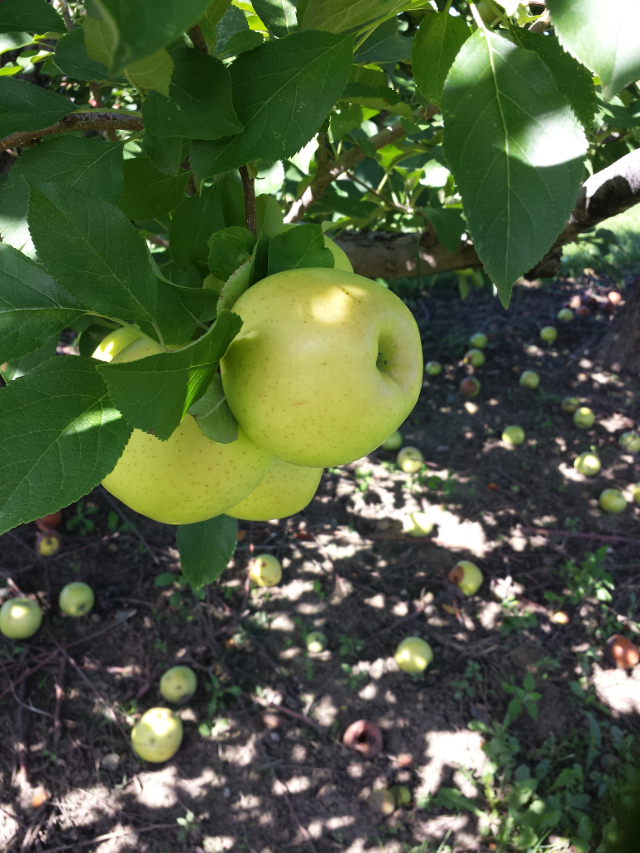
\includegraphics[width=\textwidth]{figures/active_counting/appleview1.jpg}
\end{subfigure}\quad \begin{subfigure}[t]{0.3\textwidth}
    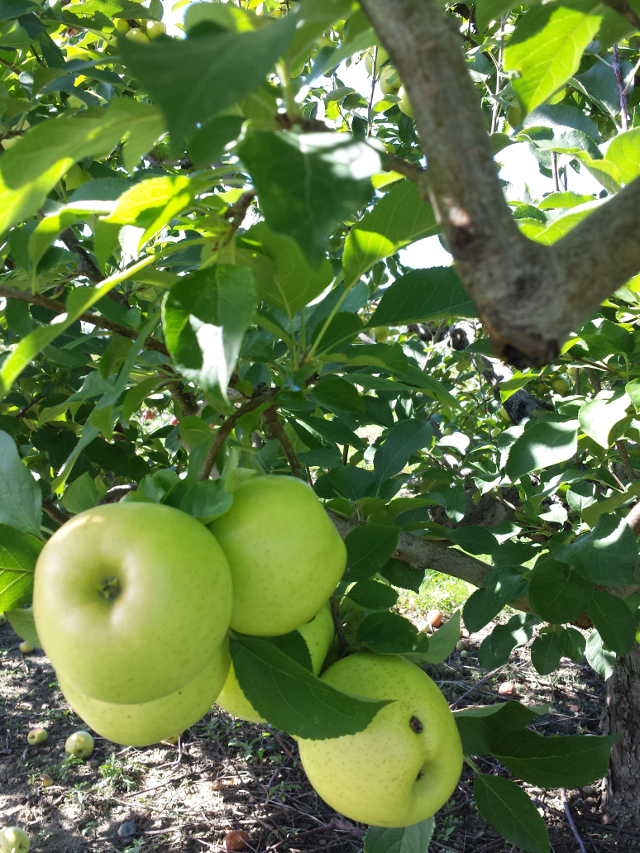
\includegraphics[width=\textwidth]{figures/active_counting/appleview2.jpg}
\end{subfigure}\quad \begin{subfigure}[t]{0.3\textwidth}
    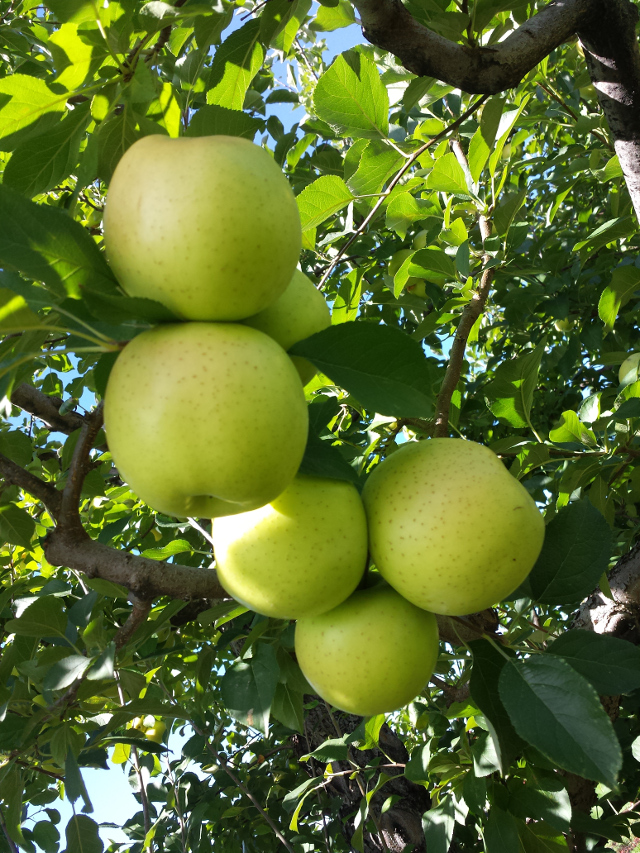
\includegraphics[width=\textwidth]{figures/active_counting/appleview3.jpg}
\end{subfigure}
        
        
        \caption[Necessity of multiple viewpoints for accurate fruit counting.]{Necessity of multiple viewpoints for accurate fruit counting. A single view of a cluster can be deceiving. The first view suggests that there are three apples, the second one suggests five and finally, from a bottom-up view, we see that there are actually six apples in the cluster.
\label{fig:compl}}
\end{figure}
\section{System Description}\label{sec:sysdes}

Our system consists of a monocular camera mounted on a robotic manipulator which is fixed on a ground robot (Fig.~\ref{fig:robotplatform}). Our long-term target is to develop algorithms enabling this platform to traverse the orchard rows autonomously and collect useful data for phenomics and precision agriculture. This chapter focuses specifically on close up view planning for fruit counting using the camera mounted on the manipulator. We assume that the camera is calibrated. The robot pose $[^w R_r|t_r]$ and the camera pose $[^w R_c|t_c]$ are known with respect to world frame $\{w\}$. From this camera $\{c\}$ mounted on a robotic manipulator $\{r\}$ and facing a fruit cluster $A$, we want to compute a sequence of viewpoints to place the camera to correctly predict the fruit count. We assume that we have a rough estimate of $\left(d_{est}\right)$ of the working distance (distance from the camera to the fruit cluster). Using this estimate, we define a viewing sphere $S$ centered at the center of $A$ and having radius $d_{est}$. As the viewing sphere is around the cluster center, we can only operate in the hemisphere facing the camera which is in the reachable workspace of the robot. We place $m$ viewpoints $V = \{v_1,v_2, \ldots, v_m\}$ in the frontal hemisphere of $S$. Fig.~\ref{fig:viewsphere} shows an example of one such viewing sphere (left image) and the viewpoints placed on it(right image). The ellipsoids inside the viewing sphere are colored randomly for clarity of understanding and have no other significance.

\begin{figure}[htb]
\centering

    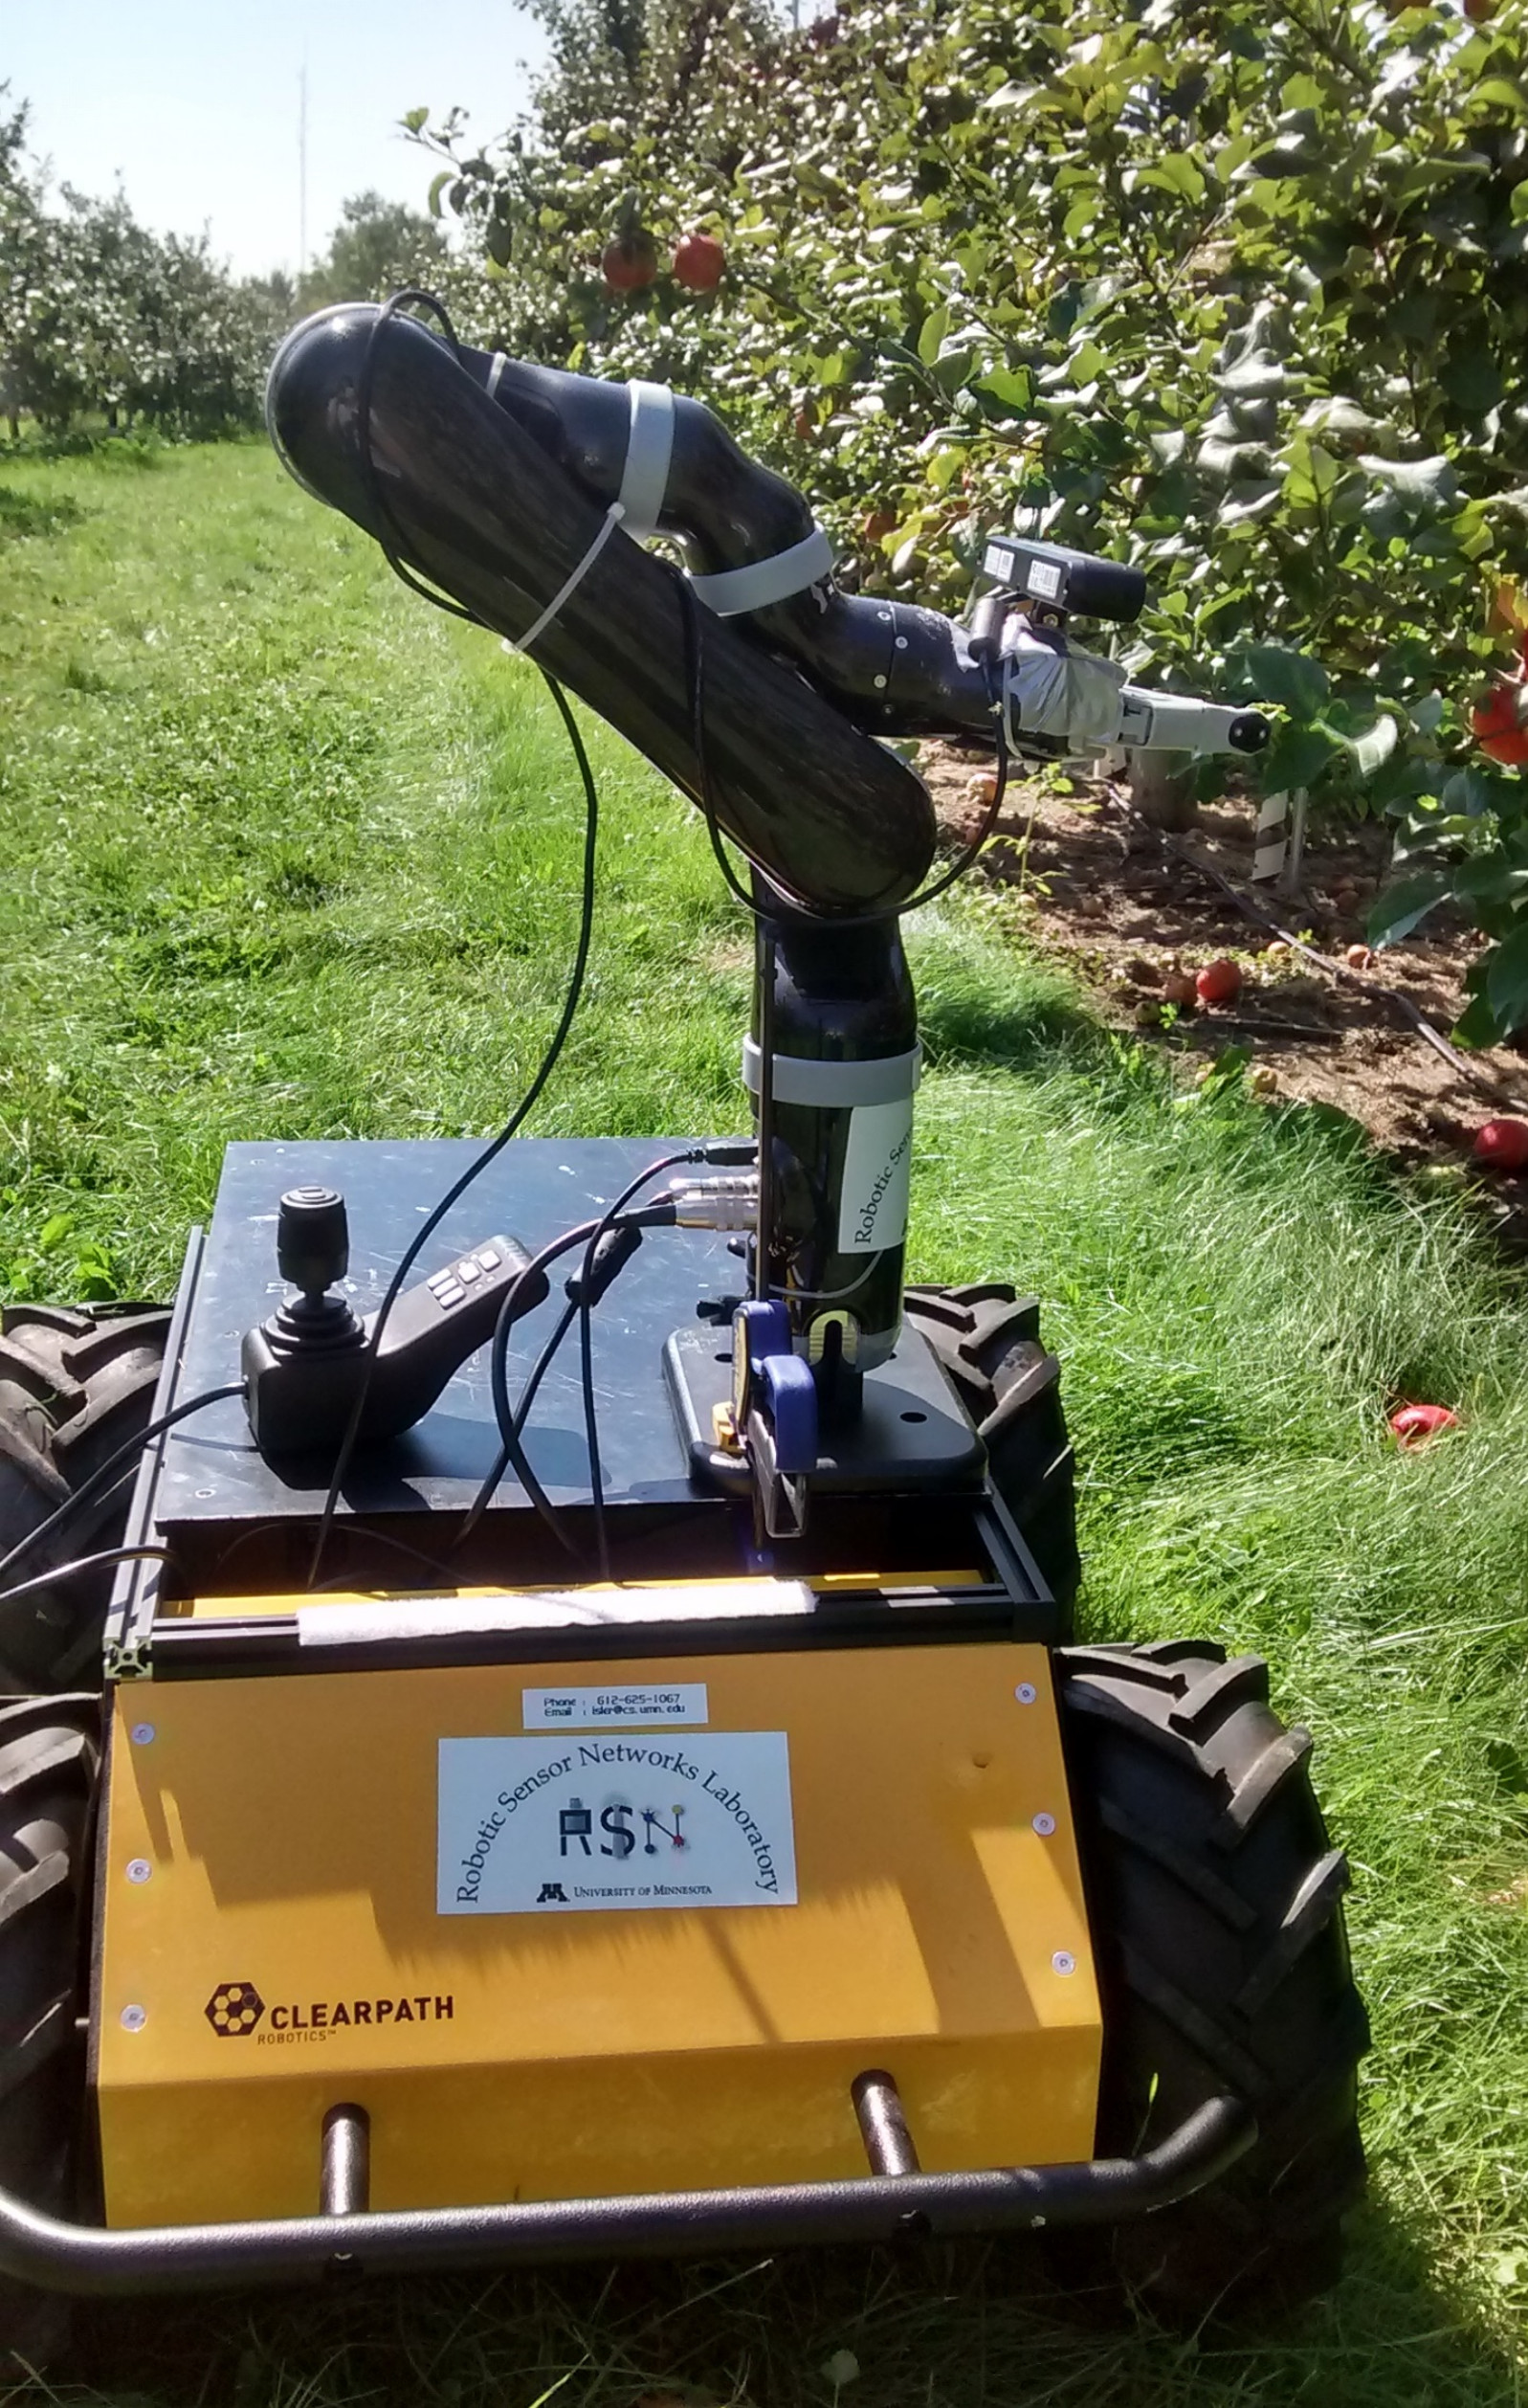
\includegraphics[scale = .1]{figures/active_counting/platform.jpg}
    \caption[Robotic platform for active perception.]{Robotic platform for automating different precision agriculture and phenomics operation}
\label{fig:robotplatform}
\end{figure}


\begin{figure}[htb]
\centering
\begin{subfigure}[t]{0.45\textwidth}
    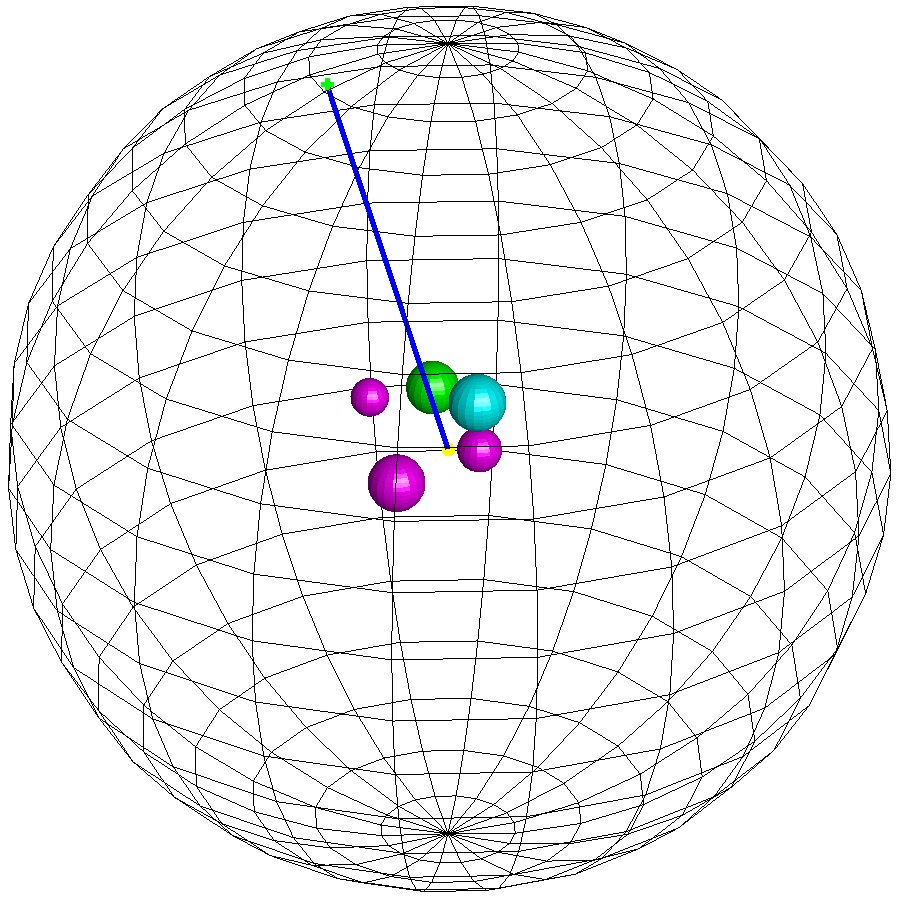
\includegraphics[width=\textwidth]{figures/active_counting/viewingsphere2.png}
\end{subfigure}\quad \begin{subfigure}[t]{0.45\textwidth}
    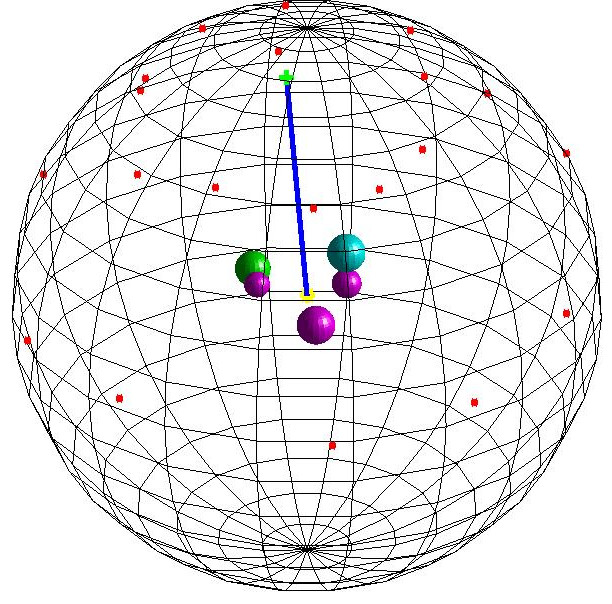
\includegraphics[width=\textwidth]{figures/active_counting/viewpoints.jpg}
\end{subfigure}
        \caption[Schematic diagram of viewing sphere and viewpoints.]{ We define the center of our viewing sphere to the perceived center of the fruit cluster under observation. The radius is set as the estimated distance from the camera to the cluster center. Figure on left shows the viewing sphere, the ellipsoidal fruit inside it (the fruit of the cluster are colored randomly for identification purposes) and the blue line joining camera center to the cluster center. Figure on the right shows the placed viewpoints (red dots).}
\label{fig:viewsphere}
\end{figure}

\section{Problem Formulation}\label{sec:probfor}
In this section, we formalize the problem definition for intra-cluster view planning. The term, ``intra-cluster'' means that at any specific time instant we are only planning views for one particular cluster. We will represent the fruit in 3D space by their enclosing ellipsoids $e$. Let $A = \{e_1,e_2, \ldots e_n \}$ represent an fruit cluster of size $n$ in world space. The condition for fruit being in a cluster is that the maximum distance between any two enclosing ellipsoids $e_i,e_j$ where $i,j\in [1,n]$ has to be bounded. As mentioned before, we assume that we have an approximate estimate of the working distance $d_{est}$ from the camera to the cluster $A$. Given this, we define our view planning problem as the following\\

\textbf{Problem Statement:} Given an initial image $I_1$ and an approximate distance from camera to the cluster $A$, compute the next best view $v_{k}$, so as to minimize the entropy of our set of world hypotheses $W$,

\begin{equation}
\begin{split}
\argmin{v_{k}} H(W|I_{v_1},I_{v_k})= \argmin{v_k} -\mathcal{P} \left(W|I_{v_1},I_{v_k}\right) \\ \log \mathcal{P} \left(W|I_{v_1},I_{v_k}\right)
\end{split}
\label{eq:probdef}
\end{equation}
where $v_k\in V$ and it is not the initial view point.




\section{Generating World Models}\label{sec:models}
In the previous section, we formulated the problem as computing a viewpoint that minimizes the entropy $H(W|I_{v_1},I_{v_k})$. Therefore, the first and most important step for our view planning strategy is generating a complete set of world hypotheses $W$. They must cover all possible geometric configurations for a maximum cluster size to ensure convergence to the correct fruit count. As we represent the fruit in SE(3) by ellipsoids, enumerating over all possible combinations of even one or two fruit is computationally prohibitive.  

Instead, we utilize a small set of combinatorial models in terms of visible and occluded fruit which does not have any position and orientation associated with it. This combinatorial representation of fruit is our main contribution for this work. We convert these models to physical world models using image-based measurements. In this section, we present the details of the world model generation procedure. We start by introducing the combinatorial world models.

\subsection{Combinatorial World Models}\label{subsec:worldmodel}
Two models are combinatorially equivalent if the number of visible and occluded fruit from the orthographic frontal view are equal. Fig.~\ref{fig:cmb}(\subref{fig:combeq}) shows two such combinatorially equivalent models. We assume that the initial view obtained by the camera is the view from the frontal plane. According to our assumption $W = \{w_1,w_2,\ldots,w_p\}$, is a set of all possible world models and  where $w_i = \{ e_1^{w_i}, e_2^{w_i},e_3^{w_i} \ldots e_n^{w_i} \}$, is a set of $n$ ellipsoids in world space where $i \in [1,p]$ and $n \in [1,\text{maxClusterSize}]$. 

We fix the cluster size $n$ and generate our world models in terms of occluded and visible fruit. Initially, we assume that each visible fruit can occlude only one other fruit. The occluded fruit cannot further occlude other fruit. Later, we show how to extend this approach to the case where occluded fruit is allowed to occlude other fruit. Under the current assumption, there are only two layers: visible and occluded. The maximum number of occluded fruit $a_{oc}$ and the minimum number of visible fruit $a_{vis}$, for cluster size $n$ and number of layers $L=2$ is

$$ a_{oc} =  \ceil*{\frac{n}{L}}$$
$$ a_{vis} = n - \ceil*{\frac{n}{L}}$$

\begin{figure}[htb]
\centering
\begin{subfigure}[t]{0.45\textwidth}
    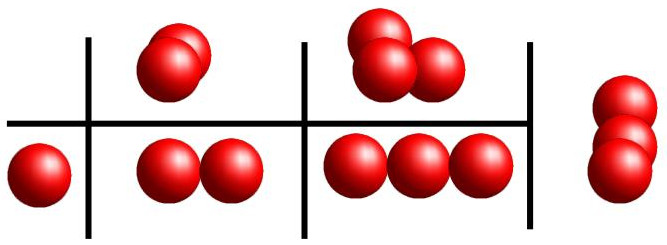
\includegraphics[width=\textwidth]{figures/active_counting/combmod.jpg}
\caption{Combinatorial models for cluster size = $3$}
\label{fig:combmodel}
\end{subfigure}\quad\begin{subfigure}[t]{0.4\textwidth}
    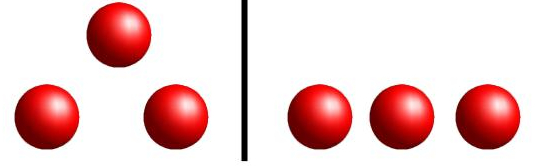
\includegraphics[width=\textwidth]{figures/active_counting/combeq.jpg}
\caption{Two combinatorially equivalent models}
\label{fig:combeq}
\end{subfigure}
\caption[Combinatorially equivalent models.]{ Combinatorial models. Fig.~(\subref{fig:combmodel}) shows the combinatorial models for clusters of maximum size three. It shows that there is six model in total with no restriction on the number of occlusion layers. If we restrict the number of occlusion level to one, the last model is eliminated. Right image shows two combinatorially equivalent views}
\label{fig:cmb}
\end{figure}


By varying the number of visible fruit (i.e the fruit in layer $1$) from $1$ to $n$ we can generate all possible models for this particular cluster size $n$. The total number of models for cluster size $n$ is actually, $\binom{L+a_{oc}-1}{a_{oc}} = a_{oc}$. In practice, this assumption of one occlusion layer (i.e $L=2$) holds for most fruit clusters.

We can easily extend the current method for the cases of multiple occlusion layers. Again, we assume that each fruit can occlude just one fruit. When the number of occluded fruit is $1$, or $n-1$ where $n$ is the cluster size, the number of models is trivially one. From the previous paragraph, we know that when the number of layers $L =2$, the total number of models is $\binom{1+a_{oc}}{a_{oc}}$. For cases where $L >2$ and $1<a_{oc}<n-1$ we find the models by using a recursive divide and conquer strategy. We subdivide occluded fruit as visible and hidden for $L\geq 2$, decrease the occlusion level by $1$ until we reach one of the base cases and combine the solutions together.

It should be noted that these models are not concerned with the actual location or size of the fruit. Their purpose is to capture the combinatorial structure of the clusters in terms of visible and occluded fruit and occlusion hierarchy. Consequently, the models only need a tag for visible/occluded and a layer number. For the rest of the chapter, we refer to these models as combinatorial world models. Fig.~\ref{fig:cmb}(\subref{fig:combmodel}) shows combinatorial world models for maximum cluster size three.
\subsection{Sensing from Individual Images}\label{subsec:singleImageCounting}
 
For predicting the next best views and to relate the combinatorial models to actual images we need to have a sensing method for individual images and actual physical models corresponding to each of the combinatorial models. For sensing from singular input images, we utilize the counting method described in Chapter~\ref{chapter:fruit_counting}. We exploit the idea of the images being generated from a two-dimensional world model (probability distribution). Each fruit in the input image is modeled by a Gaussian probability distribution function (pdf) and fruit clusters are modeled as a mixture of Gaussian. For a given image and a particular size of input clusters, this method provides us with the tentative pixel location and pixel size for each fruit and a likelihood of that cluster size being optimal. Essentially, our sensing method provides us with the likelihood of fruit being visible in the input image. In the next section, we look at how we can combine this information with the combinatorial world models and associate position and orientation to them.



\subsection{From Combinatorial Models to World Models with Position and Orientation}\label{subsec:physicalModel}

Each of our combinatorial world models contains a nonzero number of visible fruit and occluded fruit. The sensing model provides us with an estimate of the visible fruit in the image. We back project these fruit and utilize estimated depth $d_{est}$ to obtain their tentative 3D location. The sensing estimate provides only diameters across $x$ and $y$ axis. We assume the diameter of the ellipsoid along the $z$ axis is the average of the $x,y$ axis diameter. Following this procedure for all the combinatorial models, we obtain a physical model corresponding to each of the visible fruit in the combinatorial models. Now, we need to associate position and orientation to the occluded fruit. We place the occluded fruit exactly behind the visible fruit, following a left to right order. For the case of multiple level occlusion, an fruit can occupy a place in a higher occlusion level if all the corresponding places in the lower occlusion levels are filled. The sensing model provides us with the likelihood of visible fruit. To generate the likelihoods for models with occlusion we utilize the penalty and reward function described in Chapter~\ref{chapter:fruit_counting},(equation~\eqref{eq:reward},\eqref{eq:penalty}). Occluded fruit does not contribute anything to the reward function and consequently, they are just penalized for the increasing number of components. Therefore, by adding the penalty for the occluded fruit to the likelihood of the visible fruit we obtain the likelihood of the world models with occlusion. Fig.~\ref{fig:genmodel} shows an example of the generated world models for three fruit.
\begin{figure}[!htbp]
\centering

    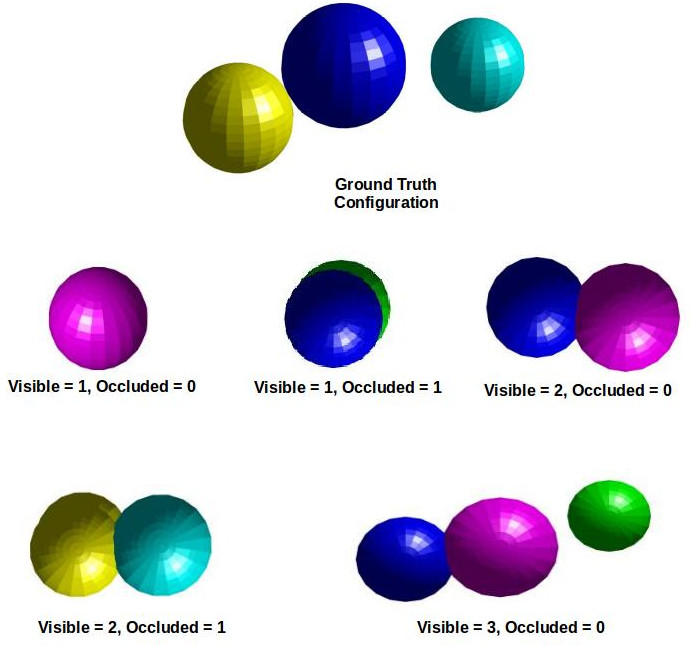
\includegraphics[width=.7\textwidth]{figures/active_counting/genmodel.jpg}

\caption[World hypotheses generated from combinatorial models for three fruit.]{ World hypotheses generated from combinatorial models for three fruit.}
\label{fig:genmodel}
\end{figure}


\section{View Planning}\label{sec:vp}

In this section, we present the details of our view planning approach. We show how to determine the next best viewpoint from the current information, how to update the posterior probabilities of the world models after each additional view and the termination criteria to be checked on each iteration. 

At each viewpoint, the camera provides us an image of the fruit cluster, $I_{v_j}(A), \text{where} v_j$ is  the $j^{\text{th}}$ viewpoint. Let, $v_1,v_2,\ldots v_k$  be the viewpoints we have chosen so far. Therefore, the next best view should be chosen so that it minimizes the entropy of the entire set of world hypotheses $W$. Equation~\eqref{eq:probdef} has the following general form

\begin{equation}
\begin{split}
\argmin{v_{k+1}}\sum_{i=1}^p -\mathcal{P} \left(w_i|I_{v_1},I_{v_2}, \ldots I_{v_k} I_{v_{k+1}}\right)& \\\log \mathcal{P} \left(w_i|I_{v_1},I_{v_2}, \ldots I_{v_k} I_{v_{k+1}}\right)
\end{split}
\label{eq:nbvf}
\end{equation}



Now we take a closer look at the term $\mathcal{P}\left(w_i |I_{v_1},I_{v_2}, \ldots I_{v_k}\right)$ and see how we can evaluate it.

\begin{equation}
\begin{split}
\mathcal{P}\left(w_i |I_{v_1},I_{v_2}, \ldots I_{v_k}\right) = \frac{\mathcal{P}\left(I_{v_1},I_{v_2}, \ldots I_{v_k}|w_i\right) \mathcal{P}\left(w_i\right)}{\mathcal{P}\left(I_{v_1},I_{v_2}, \ldots I_{v_k}\right)}\\ \approx \mathcal{P}\left(I_{v_1}|w_i\right) \mathcal{P}\left(I_{v_2}|w_i\right) \ldots \mathcal{P}\left(I_{v_k}|w_i\right) \mathcal{P}\left(w_i\right)
\end{split}
\label{eq:condapprox}
\end{equation}

In equation~\eqref{eq:condapprox}, the conditional independence of the terms of form  $\mathcal{P}\left(I_{v_k}|w_i\right)$ follows from the fact that, for a fixed world hypothesis $w_i$ the camera views depend only on $w_i$ and are independent of each other. However, for choosing the next best view (equation~\eqref{eq:nbvf}), we cannot evaluate $\mathcal{P}\left(I_{v_{k+1}}|w_i\right)$. This is because we have not yet seen $I_{v_{k+1}}$. For this case, we generate a utility value for viewpoint $v_{k+1}$ based on the expected number of occluded and visible fruit for world model $w_i$ (described in details in section~\ref{subsec:nbv}). 



\subsection{Next Best View Planning}\label{subsec:nbv}

For predicting the next viewpoint, we need to evaluate the utility of each of the possible candidate views. Let $V_c =\{ v_{k+1}, v_{k+2}, \ldots v_{k+r}\}$ be the set of candidate viewpoints. For each of this viewpoint $v_{k+j}, j\in [1,r]$, we generate an image of each of our world hypotheses $w_i$. Our physical world models consist of ellipsoids $w_i = \{ e_1^{w_i}, e_2^{w_i},e_3^{w_i} \ldots e_n^{w_i} \}$. We represent each of them in a quadric format which allows us to compute their projection quickly. While projecting, we sort the quadric by their depth order and compute the overlap between the projected ellipses. Following this procedure, we determine the visibility of each ellipsoid in the resulting image. If more than $20\%$ of a projected ellipse is not occluded by any other we mark it as visible. Performing this operation for each viewpoint $v_{k+j}$ and world model $w_i$ we can determine the visible and occluded fruit for each viewpoint for each world model $w_i$. We build two tables, $\text{visModel}, \text{occModel}$, of dimension $m \times p$ where $m$ is the total number of viewpoints and $p$ is the total number of world models. 

\begin{equation*}
\begin{split}
\text{visModel}(i,j) = \text{visible fruit generated by}\\ w_j \text{ from } v_i 
\end{split}
\end{equation*}

\begin{equation*}
\begin{split}
\text{occModel}(i,j) = \text{occluded fruit generated by }\\ w_j \text{ from view point } v_i 
\end{split}
\end{equation*}

We define the utility of a view in terms of these visibility and occlusion models by building a similar table which we refer to as the utilityModel.
\begin{equation*}
\begin{split}
\text{utilityModel}(i,j) = \frac{\text{visModel }(i,j)}{\text{occModel}(i,j) + \text{visModel }(i,j) } 
\end{split}
\end{equation*}

Following the computation of this table, we normalize the utilities across all the viewpoints to obtain a probability distribution of the utility for each world model. The next best view is found from these computed utilities. We consider two methods for this step. First, we plan for a single view that minimizes the entropy of our hypotheses set $W$. Second, we plan for a sequence of views that must be taken to verify all different configurations of visible and occluded fruit from our hypotheses set. It should be noted that regardless of the single/ multiple step planning we make one move at a time (for multiple steps - the first view in the sequence), recompute the posterior probabilities of world hypotheses and plan for the next view using the single/multiple-step method. We start with single step planning.

\begin{figure}[htb]
\centering
\begin{subfigure}[t]{\textwidth}
    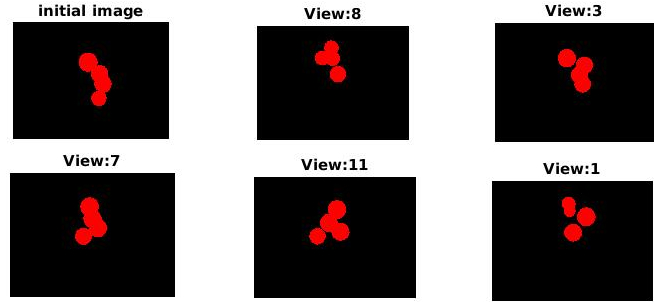
\includegraphics[width=\textwidth]{figures/active_counting/viewsgd}
\caption{Viewpoints chosen by single step view planning}
\label{fig:simviews}
\end{subfigure}\\
\begin{subfigure}[t]{\textwidth}
    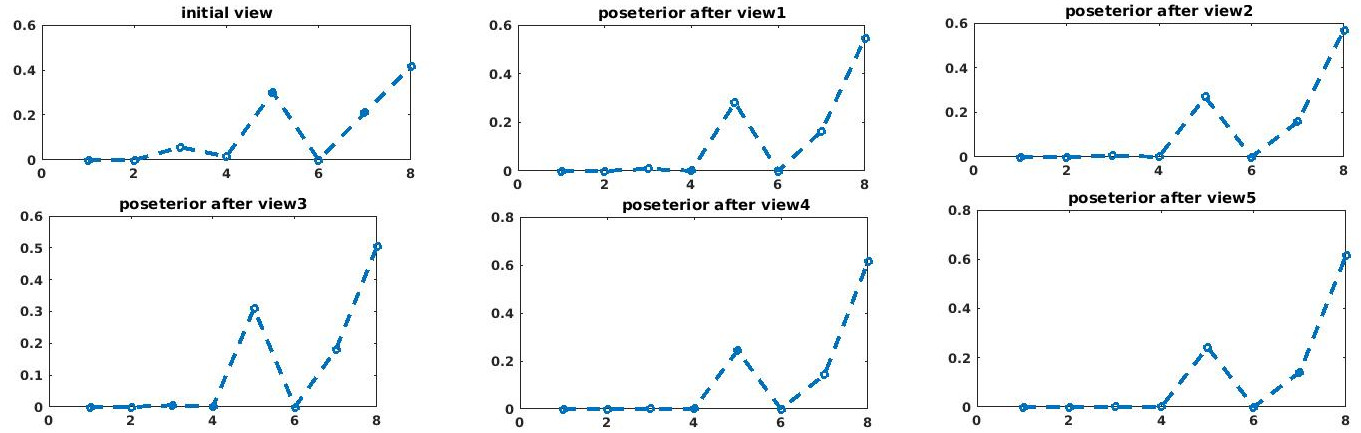
\includegraphics[width=\textwidth]{figures/active_counting/posterior1}
\caption{Posterior probability distribution of the world hypotheses}
\label{fig:simpost}
\end{subfigure}
\caption[Simulation results for single step planning.]{Sample result from simulations. We randomly generated a 3D model of four fruit. Our  multiple step view planning algorithm selected three more views before converging to a world model with correct world counts }
\label{fig:simsamp}
\end{figure}

\subsubsection{Planning Single Step at a Time}\label{subsubsec:greedy}
For single step  planning we can directly use equation~\eqref{eq:nbvf}. For any candidate view point $v_{k+1}$, and the hallucinated image $I_{v_{k+1}}$ (generated by projecting world model $w_i$ to the camera at view point $v_{k+1}$), 
\begin{equation}
\centering
\begin{split}
\mathcal{P}\left(w_i |I_{v_1},I_{v_2}, \ldots I_{v_k},I_{v_{k+1}}\right)\\ 
\approx \mathcal{P}\left(I_{v_1}|w_i\right) \mathcal{P}\left(I_{v_2}|w_i\right) \ldots \mathcal{P}\left(I_{v_k}|w_i\right)\mathcal{P}\left(I_{v_{k+1}}|w_i\right) \mathcal{P}\left(w_i\right)
\\ = \mathcal{P}\left(w_i |I_{v_1},I_{v_2}, \ldots I_{v_k},\right) \text{utilityModel}(k+1,i)
\end{split}
\label{eq:greedy}
\end{equation}
We replace this value in equation~\eqref{eq:nbvf}, after
normalizing the values across all the view points.


\subsubsection{Planning Multiple Steps}\label{subsubsec:multi}  A simple way to do, multiple-step planning is to plan a fixed number of views together. Essentially, it means considering $\binom{m}{k}$ candidates, where $k$ is the number of views to be planned together and $m$ is the cardinality of the viewpoint sets. Consequently, it involves multiplying $k-1$ additional utility values to equation~\eqref{eq:greedy} and evaluating equation~\eqref{eq:nbvf}. 

Instead of focusing on maximizing the number of visible fruit, we can uncover the geometry of all possible world hypotheses from different viewpoints. This is our second strategy for multiple-step planning. For this, we find different configurations of visible and occluded fruit from different viewpoints. Then we group the viewpoints for a particular world hypothesis $w_i$ by the number of visible fruit. Next, we find the maximum cardinality of these groups for all the world hypotheses and use this maximum cardinality $g$ as the number of views to be planned together. We generate the candidate viewpoint sequence like the previous method and evaluate them in terms of the covered configurations of visible and occluded fruit. The view sequences with the maximum score are evaluated using equation ~\eqref{eq:nbvf} and the best sequence is selected. The performance of the single and multiple step methods have been evaluated in terms of convergence and the average number of views required to converge. Fig.~\ref{fig:sim} shows the results. We see that the multiple-step method outperforms the single-step method for cluster sizes $5-9$. We explain the results further in section~\ref{sec:expresults}. 


\subsection{Updating the Posterior Probabilities of the World Model and Convergence Criterion} \label{sec:probupdate}

In this section, we discuss, how we can incorporate information from new views to our world models. Essentially, with each additional view, the posterior probabilities of our world models are updated. Suppose we have taken measurements from viewpoints $v_1,v_2,\ldots v_k$, and have chosen $v_{k+1}$ as our next measurement location. Then the posterior for world model $w_i$ is updated as follows

\begin{equation}
\begin{split}
\mathcal{P}\left(w_i|I_{v_1},I_{v_2}, \ldots I_{v_k} I_{v_{k+1}}\right) \approx \\ \mathcal{P}\left(I_{v_1}|w_i\right) \mathcal{P}\left(I_{v_2}|w_i\right) \ldots \mathcal{P}\left(I_{v_k}|w_i\right)\mathcal{P}\left(I_{v_{k+1}}|w_i\right) \mathcal{P}\left(w_i\right)
\end{split}
\label{eq:worldpostap}
\end{equation}
The exact value of the posterior is found by normalizing the likelihood across all the world models. Before we can apply equation ~\eqref{eq:worldpostap} we need to resolve one more issue. Our sensing model does not directly provide the quantities of the form $\mathcal{P}\left(I_{v_{k}}|w_i\right)$. Instead, it provides the likelihood of a certain number of fruit being visible in the input image. For the particular world model under consideration, we need to find the expected number of visible fruit from the visibility model that was constructed in the previous section. After this step, we can associate the sensing likelihoods with $\mathcal{P}\left(I_{v_{k}}|w_i\right)$



We use the reduction in posterior entropy coupled with the difference between the successive peaks of the posterior as our termination criteria. If the change in entropy for posterior probabilities of the world models falls below a threshold or if the difference between the successive peaks of the posterior world probabilities is above a threshold we terminate the method and pick the world model configuration with highest posterior probability. 


\section{Experimental Results}
To verify our algorithms, we conducted tests both in simulations and an indoor environment.  Indoor experiments were arranged by using a realistic artificial apple tree (Fig.~\ref{fig:expsetup}). For both simulation and indoor environments we assume that the fruit detection problem has been solved (i.e. we can locate fruit clusters in the input image). As currently there exists no method for actively planning views for counting apples, we compared our results against a lower bound provided by orthographic cameras. We also compared the performance of the single and multi-step view planning strategy.
\subsection{Comparison with Lower Bounds from an Orthographic Camera Using Cardinal Views}\label{subsec:lowerbound}
An orthographic camera can unfold the visible geometry of any object with six cardinal views: front, back, top, bottom, right and left. These views are often used in engineering drawings to capture the scale of objects. Essentially, an orthographic camera can compute the number of fruit (visible from at least one view) in any cluster size with six views maximally. Given a fixed cluster size, we use the number of views required by an orthographic camera to be the lower bound for the number of views. For single fruit, two perpendicular views are necessary to make sure that there is only a single apple. For two fruit, we need three mutually perpendicular views, for three and four fruit we need four and five views. For five or more fruit six cardinal views are required. For orthographic cameras this bound is tight.
\subsection{Simulation Results }\label{subsec:simulation}
We developed a simulation system using MATLAB for testing purposes. We use sets of randomly generated ellipsoids as the fruit and simulate a camera with $40\,^{\circ}$ field of view for capturing the images. To simulate the estimated depth from the camera to the fruit cluster we added Gaussian noise to the actual distance($\sigma = 1, \mu = 0$). Using the estimated distance and estimated cluster center from image-based measurements we define a viewing sphere (Fig.~\ref{fig:viewsphere}. Then $25$ viewpoints are placed in the frontal hemisphere facing the camera. Using our world model generation procedure described in section~\ref{sec:models}, we generate a set of world hypotheses $W$ and predict the next best viewpoints using single step and multiple step planning strategies. Here, we present simulation results for cluster size ranging from $[1,10]$. We created $20$ instances for each cluster size and computed the number of views required to converge for the single-step and multiple-step strategies. Fig.~\ref{fig:sim} shows the comparison of the single-step and multiple-step strategy along with the orthographic lower bound and convergence plot. We see that the multiple-step planner outperforms the single-step planner for cluster sizes $5-9$ (Fig.~\ref{fig:sim}(\subref{fig:simview})). We see that for the large cluster sizes both planners have a higher chance of converging to wrong cluster size. This is attributed to our sensing model. In our previous work~\cite{roy2016counting} we showed that the accuracy of the likelihoods provided by our sensing model drops with increasing cluster size. However, in practice large clusters are not very common and therefore handling them with $90\%$ convergence is quite acceptable.

\begin{figure}[!htbp]
\centering
\begin{subfigure}[t]{.48\textwidth}
    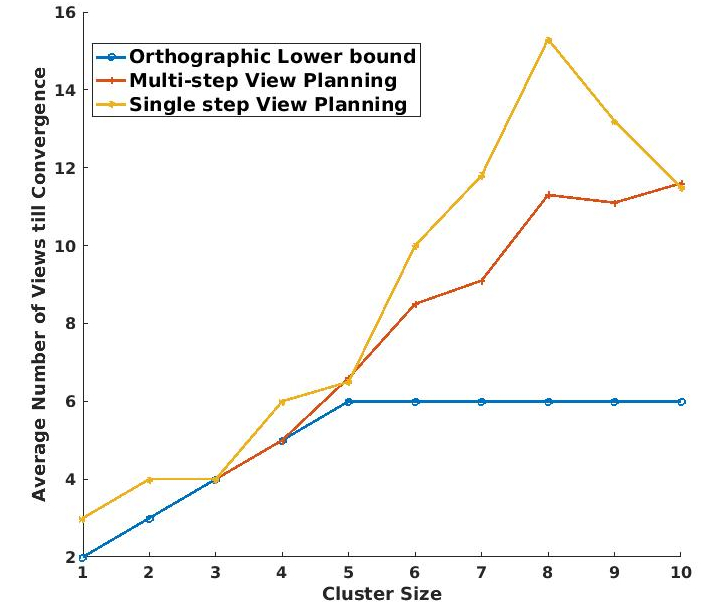
\includegraphics[width=\textwidth]{figures/active_counting/simview.jpg}
\caption{Comparison of single step and multi-step view planning with orthographic lower bound}
\label{fig:simview}
\end{subfigure}
\begin{subfigure}[t]{.48\textwidth}
    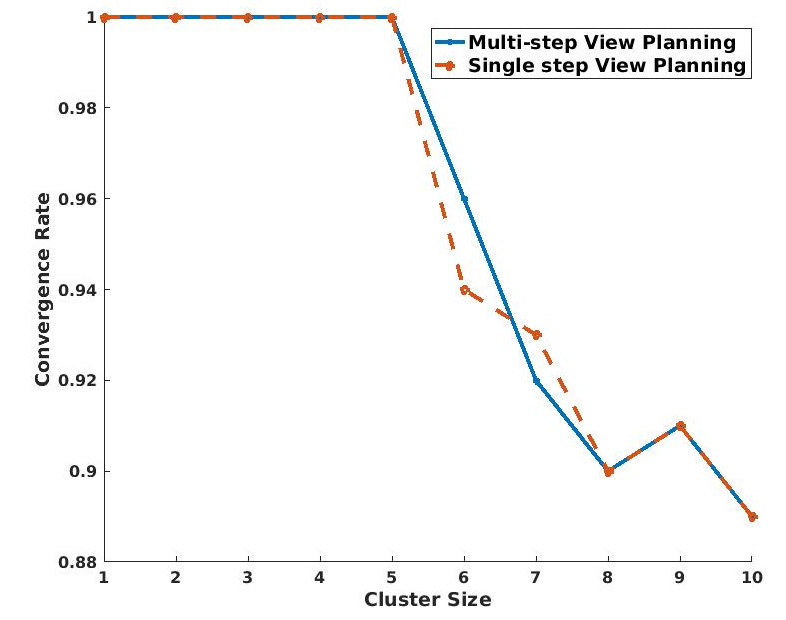
\includegraphics[width=\textwidth]{figures/active_counting/simcon.jpg}
\caption{Convergence to the correct world model}
\label{fig:simcon}
\end{subfigure}
\caption[Simulation results - comparison with orthographic lower bound and average number of views for convergence.]{Simulation results - comparison with orthographic lower bound and average number of views for convergence.}
\label{fig:sim}
\end{figure}

\begin{figure}[htb]

\begin{subfigure}[t]{0.42\textwidth}
    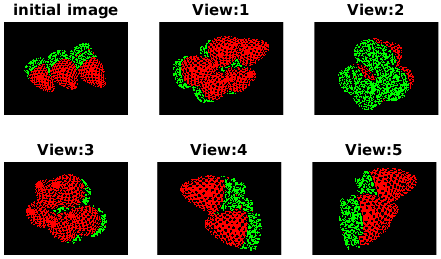
\includegraphics[width=\textwidth]{figures/active_counting/strviewfin.png}
\end{subfigure}\quad \begin{subfigure}[t]{0.53\textwidth}
    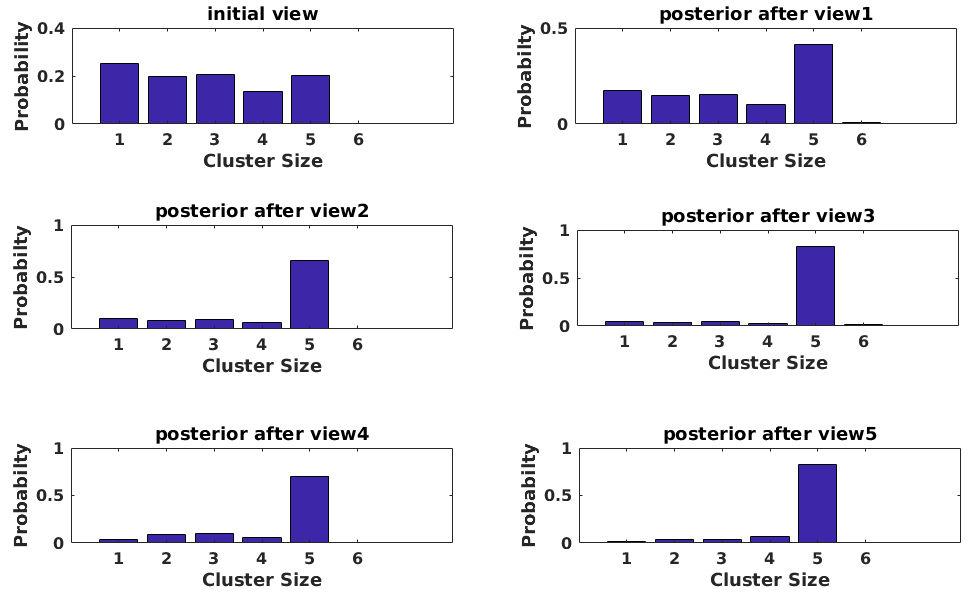
\includegraphics[width=\textwidth]{figures/active_counting/strpostfin.png}\end{subfigure}
\caption[Simulation using 3D models of strawberries]{Simulation using 3D models of strawberries.Left images show the views obtained by the camera. On the right, we see how the posterior distribution changes with each view. After five additional views, the greedy method converges.}
\label{fig:sim3d}
\end{figure}

\subsection{Indoor Experiments}\label{subsec:indoor}
In the indoor experiments, we use an artificial apple tree and synthetic apples. Fig.~\ref{fig:indoorexp} shows our experimental setup and how our algorithm performs in one of the experiments. The cluster under observation (Fig.~\ref{fig:indoorexp}(\subref{fig:indoorviews})) has three apples, but none of the views shows all of them. Our multi-step planning algorithm plans the views required and converges to the correct world model containing three apples in four views.
\begin{figure}[!htbp]
\centering
\begin{subfigure}[b]{.32\textwidth}
    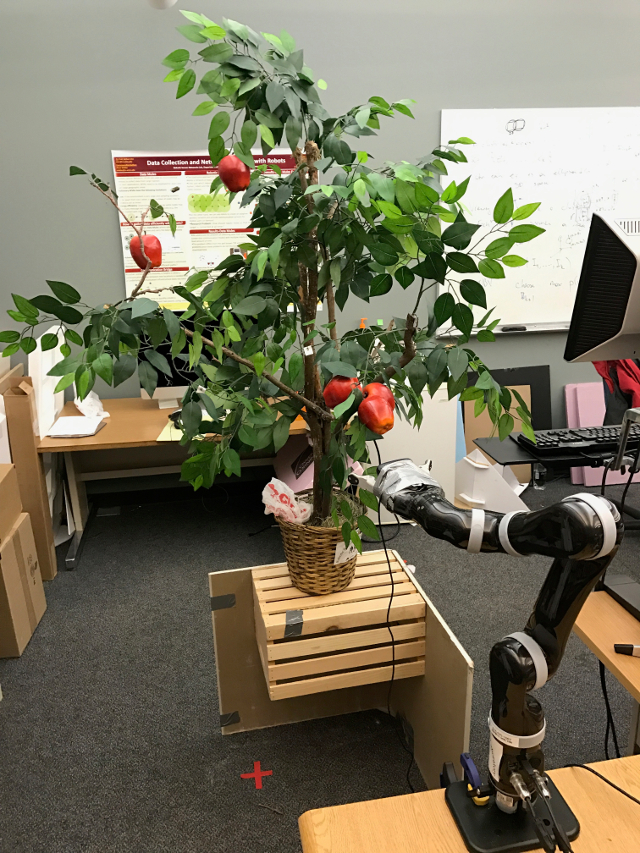
\includegraphics[width=\textwidth]{figures/active_counting/expsetup.jpeg}
\caption{Experimental Setup}
\label{fig:expsetup}
\end{subfigure}\quad \begin{subfigure}[b]{.58\textwidth}
    \begin{subfigure}[b]{\textwidth}
        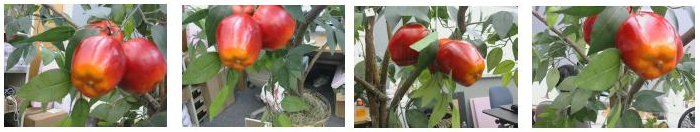
\includegraphics[width=\textwidth]{figures/active_counting/realexppics.jpg}
    \caption{Planned Views. None of them shows all three apples clearly.}
    \label{fig:indoorviews}
    \end{subfigure}\\
    \begin{subfigure}[b]{\textwidth}
        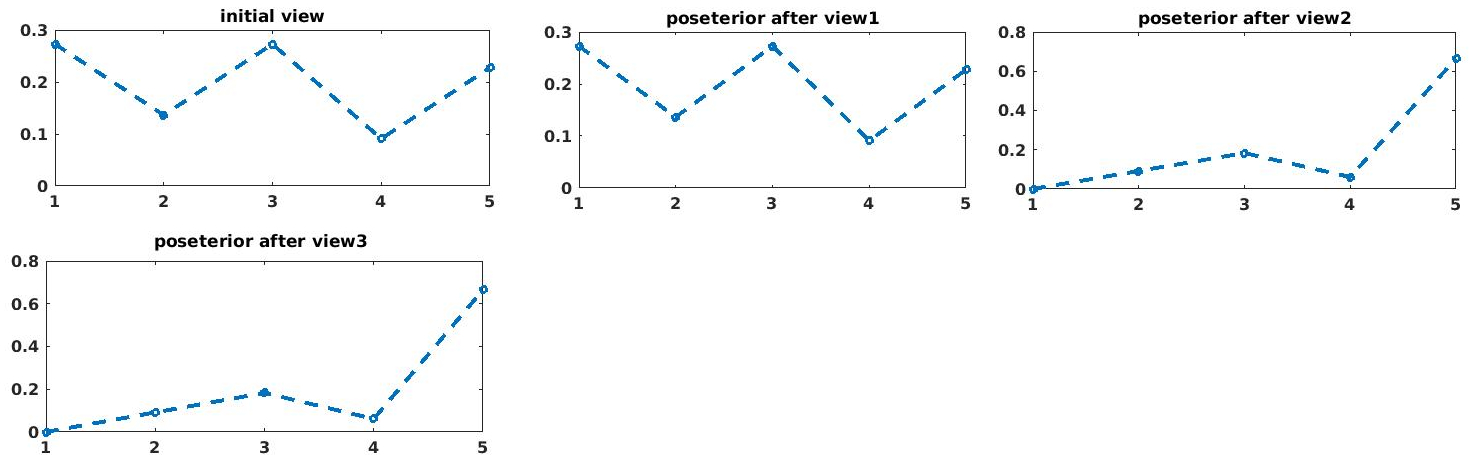
\includegraphics[width=\textwidth]{figures/active_counting/realexppost2.jpg}
    \caption{Posterior Probabilities of the World Model. The configuration of visible and hidden apples in the models $\{1,2,3,4,5\}$ are $\{(1,0),(1,1),(2,0),(3,0),(2,1)\}$}
    \label{fig:indoorposterior}
    \end{subfigure}
\end{subfigure}
\caption[Indoor Experiments]{ Indoor Experiments}
\label{fig:indoorexp}
\end{figure}


\section{Limitations and Conclusion}

In this chapter, we considered a view planning task where the goal is to choose views so as to accurately estimate the fruit count in a cluster. This task appears in agriculture automation applications such as yield mapping, fruit thinning and close-up inspection. We presented an approach where each fruit is represented as an ellipsoid. The number of ellipsoids, as well as their parameters (location and dimensions), constitute a world hypothesis. Rather than enumerating all possible world hypotheses, which is computationally prohibitive, we show how combinatorially distinct world hypotheses (regarding the visibility relationship between the apples) can be enumerated. Based on this we designed single and multi-step planners which were evaluated both in simulation and in an indoor experimental setup. Our results indicate that for larger cluster size $5-9$ the multi-step planner performs better than the single-step planner. The discussed approach was tested on apple clusters containing $10-14$ apples and the convergence rate was around $90\%$. 

Though the approach successfully converges to the correct count, it often fails to uncover the correct geometry of the clusters and takes more views than required to converge. This is due to the fact that with each additional view we only update the posterior probabilities of each combinatorial world models but the underlying physical models (generated from the initial view) are not updated. Incorporating this update will help us find the precise geometric representation of the cluster and converge quickly. After converging to the correct geometric configuration, the precise locations of the fruit ellipsoids can be obtained using ten or more point correspondences between two or more views~\cite{cross1998quadric}. 

Additionally, we need to plan views differently for different kinds of fruit. For example, strawberries and raspberries do not form large clusters but the space between individual fruit/ fruit cluster is very small. Therefore, inter-cluster views are going to be far more effective than intra-cluster views. On the other hand, blueberries often form large clusters and our intra-cluster view planning is going to be more effective in that case.


